\chapter{Wstęp}
\label{cha:wstep}

Obecny rozwój mikroprocesorów, pozwala na tworzenie coraz bardziej złożonych urządzeń. Rozwój układów o niskim zużyciu energii, popycha elektronikę w kierunku małych, wielofunkcyjnych urządzeń. Połączenie tych dwóch procesów pozwala na stworzenie elastycznych urządzeń, których zastosowanie może zmieniać się jedynie dzięki oprogramowaniu.

%---------------------------------------------------------------------------

\section{Cele pracy}
\section{Analiza wymagań technicznych i dobór komponentów}
\label{sec:technical_analysis}

Planując pracę, zdecydowano się wykorzystać trzy moduły:
\begin{itemize}
    \item A
    \item B
    \item C
\end{itemize}
\subsection{A}
\subsubsection{B}

\begin{figure}[h]
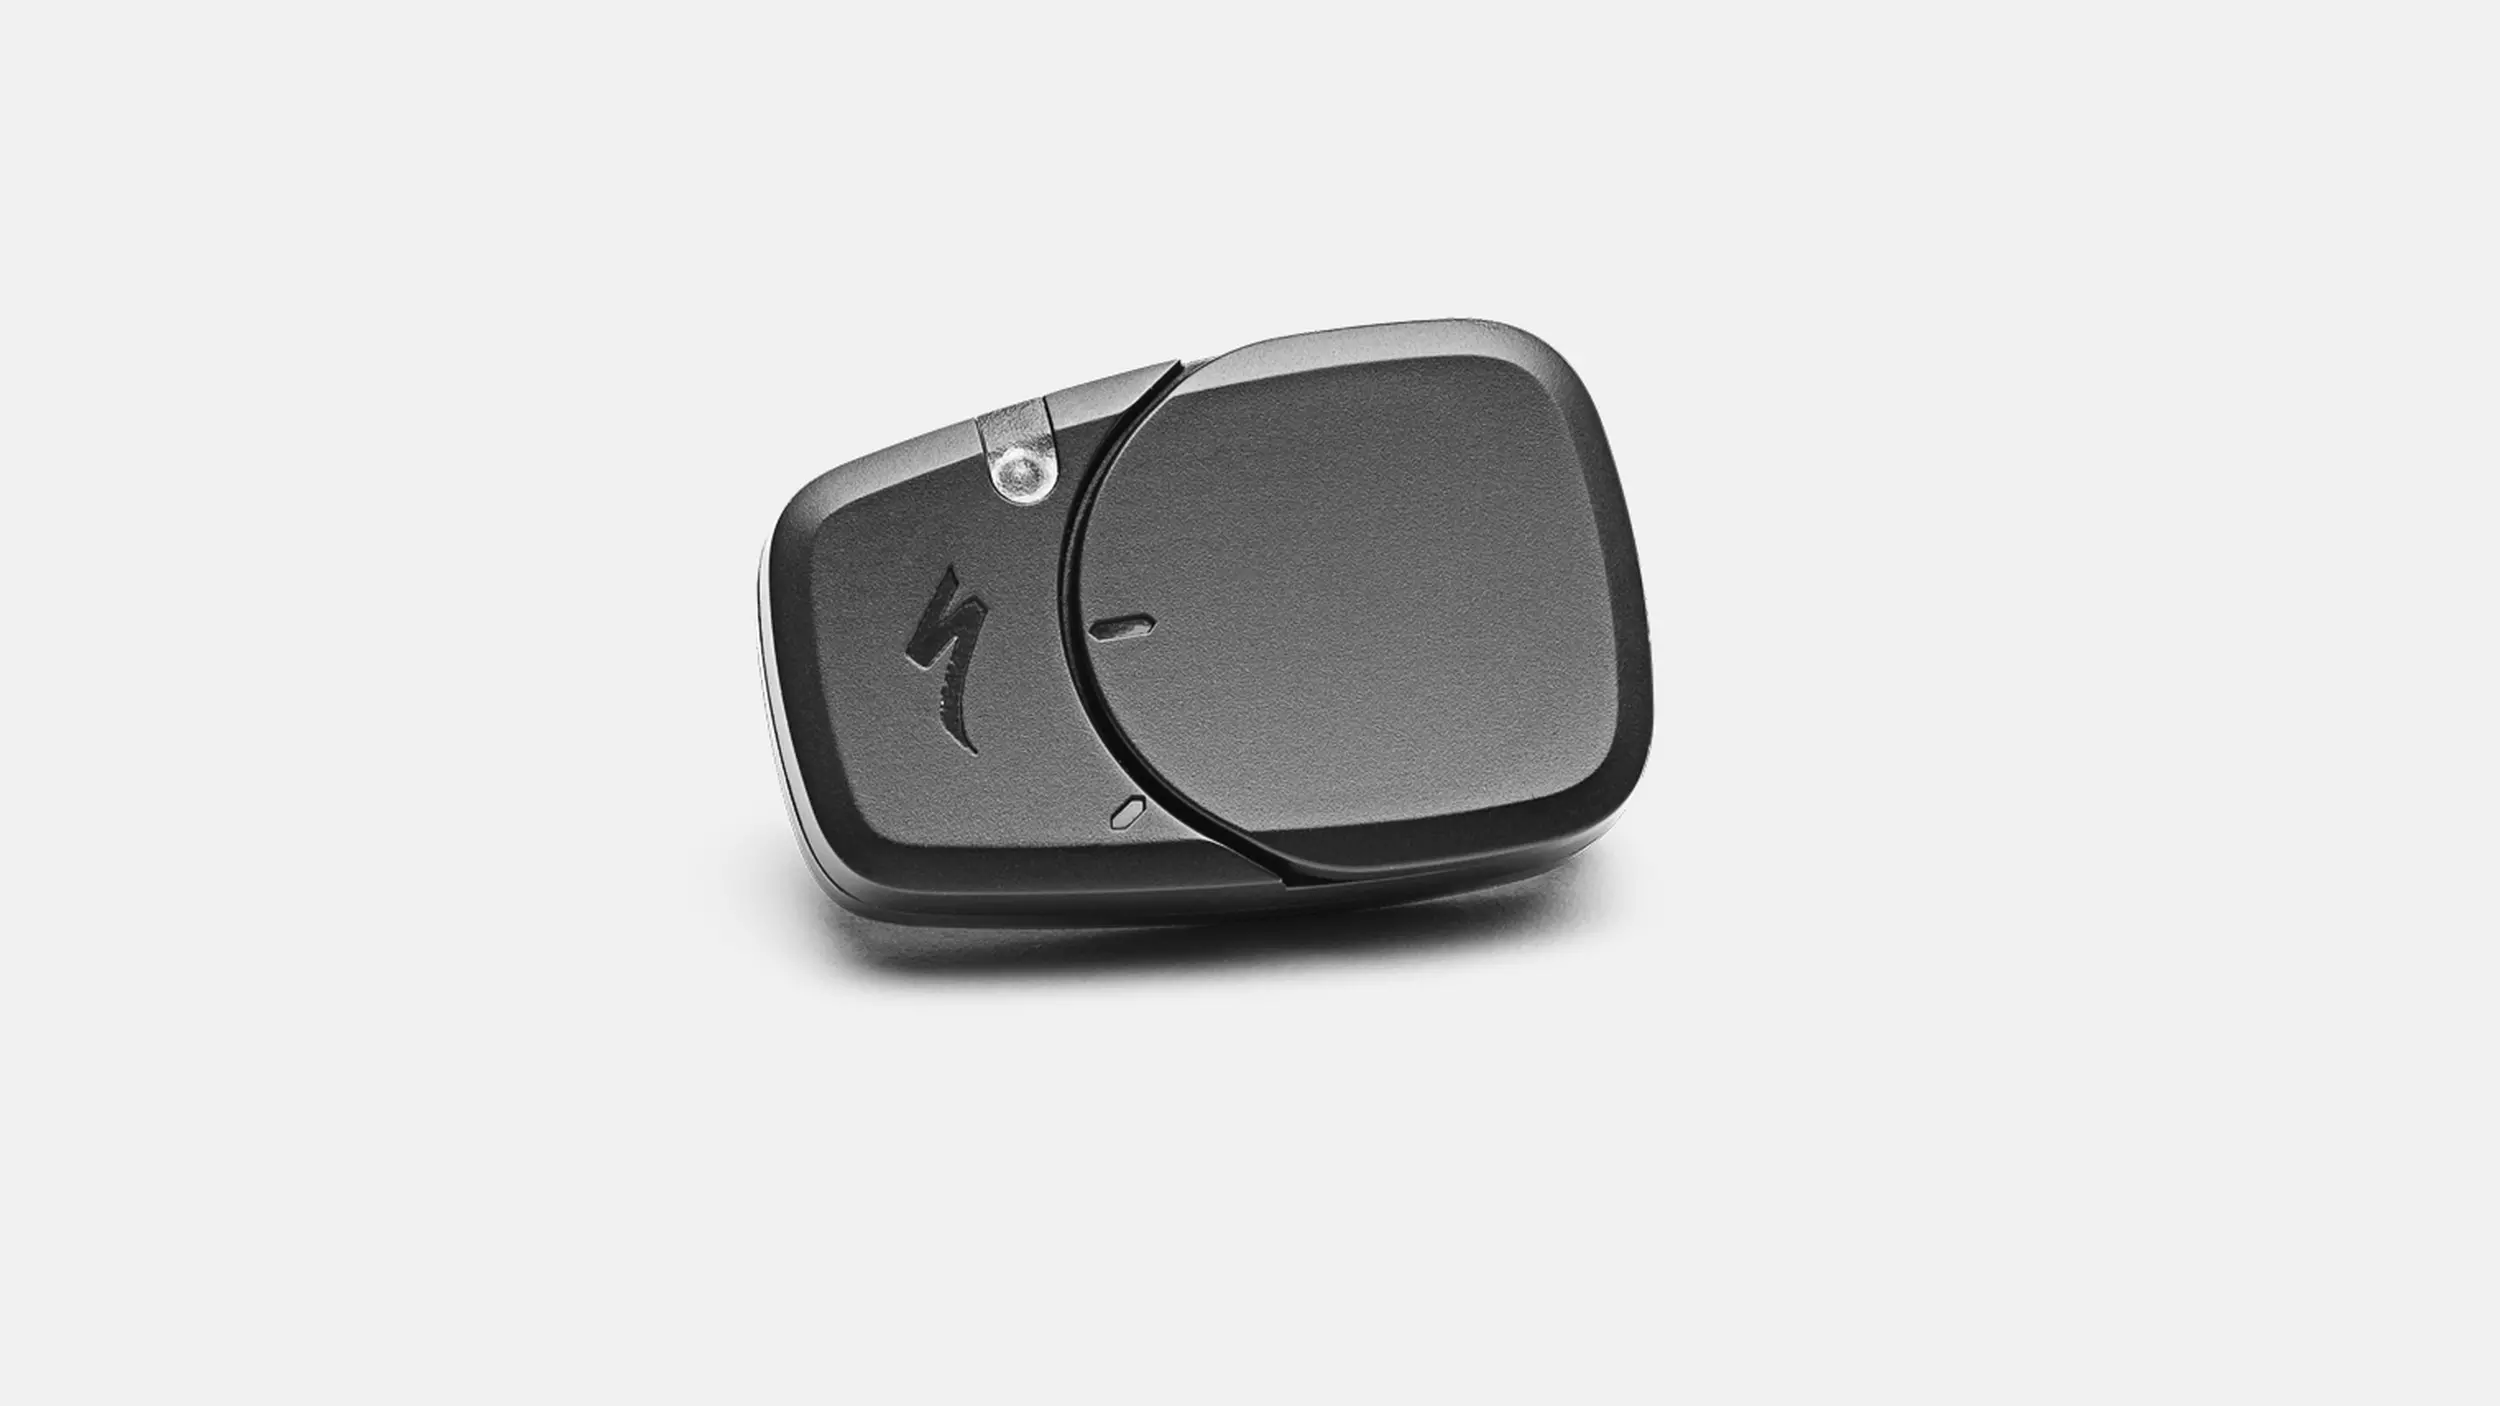
\includegraphics[width=7cm]{Graphics/angi.png}
\centering
\caption{Urządzenie ANGI, stworzone przez firmę Specialized \cite{ANGI}}.
\centering
\label{img:angi_img}
\end{figure}

%---------------------------------------------------------------------------














